Da teoria à prática, a maior dificuldade. De entre as diferentes abordagens, após alguma pesquisa, ficamos pela {\bf Geométrica}, pelo simples facto de não existir desvantagens notáveis face às restantes. Deste modo o View Frustum Culling está implementado para balas, torres e árvores.

\section{Bounding Spheres}
Está claro que \textit{axis aligned bounding boxes} é uma melhor implementação que \textit{bounding spheres} uma vez que permite criar uma menor margem de erro para casos de objectos no limite do frustum. No entanto trata-se de um jogo com poucos objectos onde a diferente margem de erro não será significativa e como tal \textit{bounding spheres} são a melhor escolha vez que apresentam o mesmo resultado e mais fácil implementação.


\begin{lstlisting}[caption=Método para teste com \textit{bounding spheres}.]
int Frustum::sphereInFrustum(Vertex *p, float raio) {

    int result = INSIDE;
    float distance;

    for (int i = 0; i < 6; i++) {
        distance = pl[i].distance(p);
        if (distance < -raio)
            return OUTSIDE;
        else if (distance < raio)
            result = INTERSECT;
    }
    return (result);

}
\end{lstlisting}

\begin{figure}[here]
                 \centering{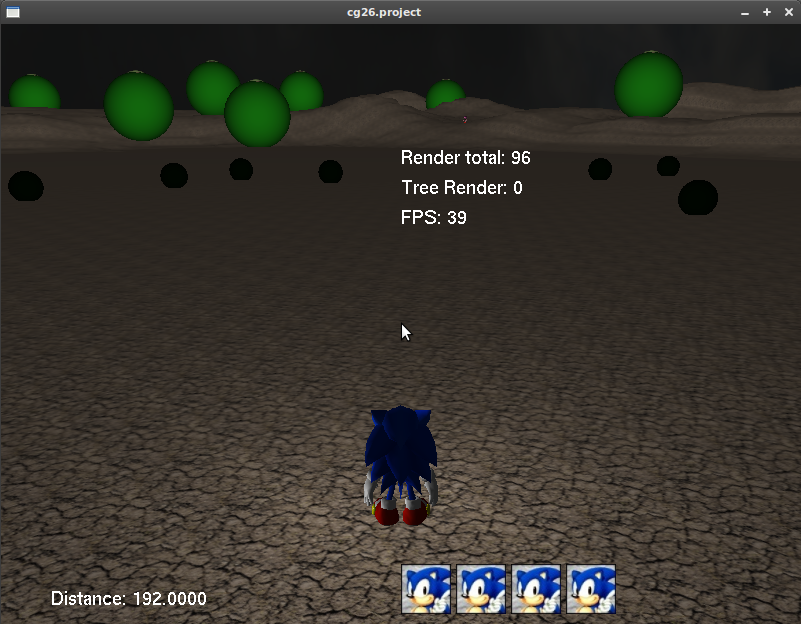
\includegraphics[width=0.8\textwidth]{images/frustum.png}}
                 \caption{Implementação de \textit{bounding spheres}.}
                 \label{fig:prototype}
\end{figure}
